\section{Results\label{sec:ch8:results}}

\begin{table}
\centering
\small

\begin{subfigure}[b]{\textwidth}
\centering
\caption{Maximum control and optimal plant variables.}
\begin{tabular}{ccccccc}
\hline \hline 
\# & Figure & $\Psi_a/w_a$ & $\Psi_d$ & $w_1 \left( y_1 - z_0 \right)^2$ & $w_2 y_2^2$ & $w_3 y_4^2$ \\
\hline 
1 & Fig.~\ref{fig:ch8:csuspension1} & 2 & 10.96 & 6.60 & 4.36 & 0.00 \\
2 & Fig.~\ref{fig:ch8:csuspension2} & 1 & 7.79 & 3.10 & 1.51 & 3.18 \\
3 & Fig.~\ref{fig:ch8:csuspension3} & 3 & 7.52 & 3.25 & 1.99 & 2.28 \\
4 & Fig.~\ref{fig:ch8:csuspension4} & 4 & 7.79 & 3.09 & 1.51 & 3.19 \\
5 & Fig.~\ref{fig:ch8:csuspension5} & 7 & 6.58 & 2.48 & 2.43 & 1.68 \\
6 & Fig.~\ref{fig:ch8:csuspension6} & 7 & 9.69 & 5.27 & 4.42 & 0.00 \\
\hline \hline 
\end{tabular}
\end{subfigure}%

\vspace{2px}

\begin{subfigure}[t]{\textwidth}
\centering
\caption{Maximum control and optimal plant variables.}
\begin{tabular}{cccccccccc}
\hline \hline 
\# & Figure & $\max{\abs{u}}$ & $k_1$ & $k_2$ & $k_3$ & $b_1$ & $b_2$ & $m_1$ & $m_2$ \\
\hline 
1 & Fig.~\ref{fig:ch8:csuspension1} & 0 & $1.77\textsc{e}4$ & $-$ & $-$ & $1.88\textsc{e}3$ & $-$ & $-$ & $-$ \\
2 & Fig.~\ref{fig:ch8:csuspension2} & 598 & $-$ & $-$ & $-$ & $-$ & $-$ & $-$ & $-$ \\
3 & Fig.~\ref{fig:ch8:csuspension3} & 634 & $1.47\textsc{e}4$ & $-$ & $-$ & $1.00\textsc{e}3$ & $-$ & $-$ & $-$ \\
4 & Fig.~\ref{fig:ch8:csuspension4} & 611 & $6.89\textsc{e}6$ & $-$ & $-$ & $6.04\textsc{e}5$ & $-$ & $1.02\textsc{e-}3$ & $-$ \\
5 & Fig.~\ref{fig:ch8:csuspension5} & 478 & $9.55\textsc{e}4$ & $6.67\textsc{e}3$ & $8.83\textsc{e}4$ & $1.46\textsc{e}4$ & $2.01\textsc{e}3$ & $3.11\textsc{e-}3$ & $-$ \\
6 & Fig.~\ref{fig:ch8:csuspension6} & 0 & $7.28\textsc{e}4$ & $8.54\textsc{e}3$ & $2.51\textsc{e}5$ & $1.00\textsc{e}3$ & $2.27\textsc{e}3$ & $3.21\textsc{e}0$ & $1.10\textsc{e}0$ \\
\hline \hline 
\end{tabular}
\end{subfigure}%

\caption{Summary of the suspension design results.\label{fig:ch8:results}}

\end{table}

In this section, we summarize the results of the vehicle suspension case study.
We utilize the code from Ref.~\cite{github-dt-qp-project} to solve the control subproblem.
The defect constraints are formed using the \glsfoo[noindex]{TR} and the chosen quadrature the \glsfoo[noindex]{CQHS} method (see Chapter~\ref{ch:5}).
It was determined that 2000 time points were needed to approximate sufficiently the problem.
The results for the first four architectures in Fig.~\ref{fig:ch8:suspensions} are presented in Table~\ref{fig:ch8:results}, along with the other two novel candidate suspensions.
A variety of stochastically generated suspensions were evaluated in the graph structure space defined by Prob.~(\ref{eq:ch8:CRP}), and the two reported novel architectures were the among the best performing for an active or passive suspension system.

% new paragraph
As expected, the worst-performing suspension of the six in Fig.~\ref{fig:ch8:suspensions} was the canonical passive design (some of the optimal position trajectories and the rattlespace are shown in Fig.~\ref{fig:ch8:results1}).
Here we see fairly large fluctuations in $z_{\xcolor{S}}$, and the rattlespace constraint is satisfied. 
The alternative passive suspension in Fig.~\ref{fig:ch8:csuspension6} (results in Fig.~\ref{fig:ch8:results6}) achieved a 12\% reduction in the objective function.
The primary improvement was in the handling objective.
However, this architecture is more complex with seven additional components compared the original two.

% new paragraph
The results for the pure active suspension are shown in Fig.~\ref{fig:ch8:results2}.
Compared to the passive suspensions, the performance index is significantly lower, demonstrating the potential value of an active component.
Since there are no passive components naturally keeping the sprung mass near the equilibrium position in this architecture, we see a drift in the sprung mass position (but the rattlespace constraint is still satisfied).
The canonical active suspension in Fig.~\ref{fig:ch8:csuspension3} does not have this issue. 
From the results in Fig.~\ref{fig:ch8:results3}, we see a very different profile for $z_{\xcolor{S}}$.
Since this architecture has some plant design flexibility, we expected an improvement in performance over the pure active design.
A 3.5\% decrease in the objective function value is observed indicating that the addition of the two passive components does result in a minor improvement in performance.
The distribution of the individual objective function terms in Eqn.~(\ref{eq:ch8:susobj}) is quite different between the two suspensions.

% new paragraph
The addition of the dynamic absorber to the pure active suspension in Fig.~\ref{fig:ch8:csuspension4} is supposed to improve handling without compromising the comfort objective \cite{Hrovat1993a}.
However, the results in Fig.~\ref{fig:ch8:results4} indicate no performance benefit for this architecture change with respect to the specific problem parameters used in this study.
This is most readily observed with the value of the additional mass  near the lower bound of 0.001 kg (effectively removing it from the system).
It is also the only architecture where the rattlespace constraint is active at some point during the time horizon.
The final architecture had the best overall performance with a 13\% reduction compared to the canonical active suspension.
The results are shown in Fig.~\ref{fig:ch8:results6}, and this design had the smallest maximum control effort.
Once again, the dynamic absorber subcomponent (now attached to the sprung mass) is ineffective with a mass value near the lower bound.
This design did need seven additional components to achieve this performance improvement.

\begin{figure}

\begin{subfigure}[b]{0.5\textwidth}
\centering
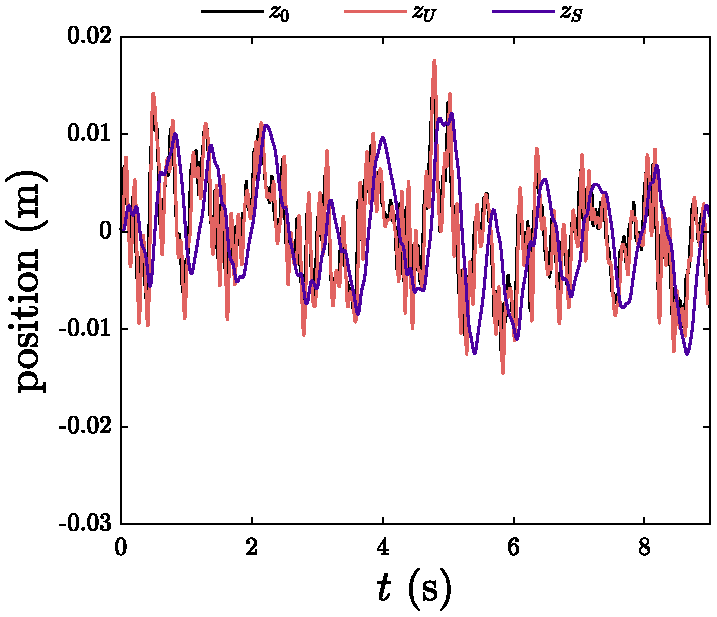
\includegraphics[width=\textwidth]{../ch8/figures/design3-position}
% 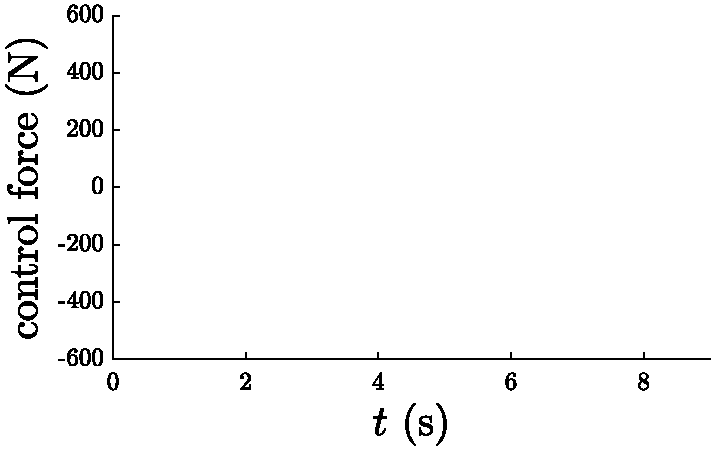
\includegraphics[width=\textwidth]{../ch8/figures/design3-control}
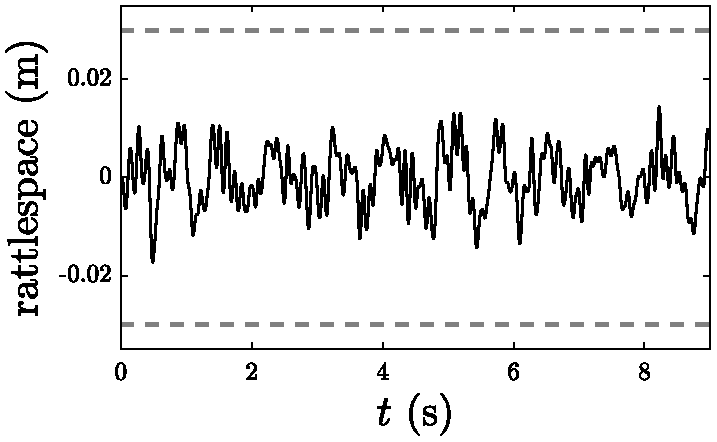
\includegraphics[width=\textwidth]{../ch8/figures/design3-rattlespace}
\caption{Canonical passive in Fig.~\ref{fig:ch8:csuspension1}.\label{fig:ch8:results1}}
\end{subfigure}%
\begin{subfigure}[b]{0.5\textwidth}
\centering
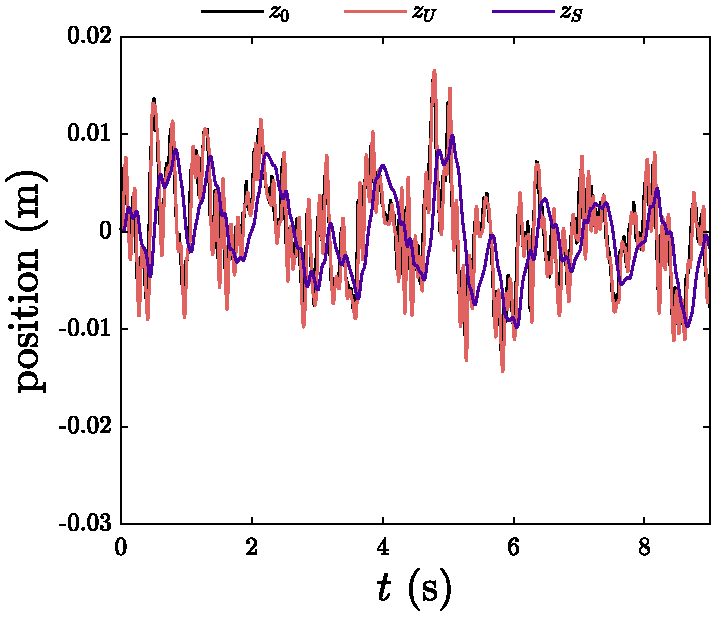
\includegraphics[width=\textwidth]{../ch8/figures/design6-position}
% 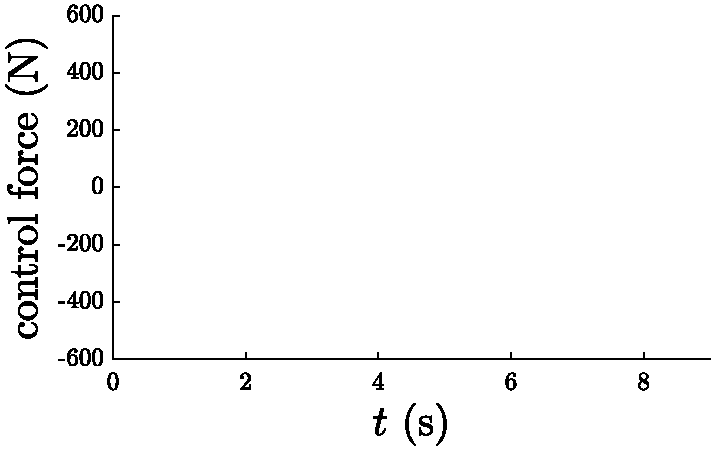
\includegraphics[width=\textwidth]{../ch8/figures/design6-control}
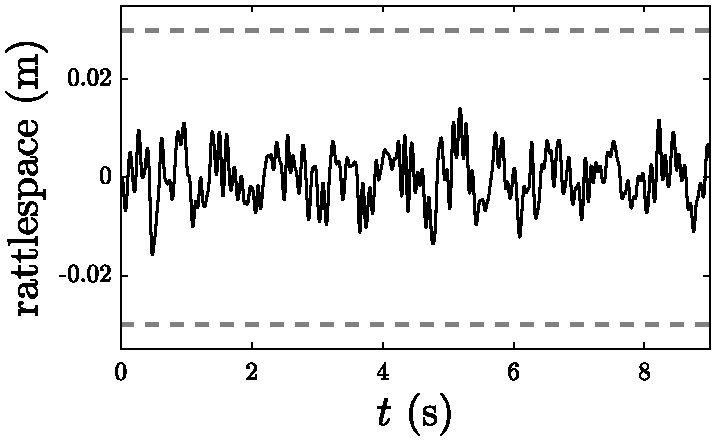
\includegraphics[width=\textwidth]{../ch8/figures/design6-rattlespace}
\caption{Passive candidate in Fig.~\ref{fig:ch8:csuspension6}.\label{fig:ch8:results6}}
\end{subfigure}%

\caption{Optimal trajectories for the two passive suspensions.}

\end{figure}

\begin{figure}

\begin{subfigure}[b]{0.5\textwidth}
\centering
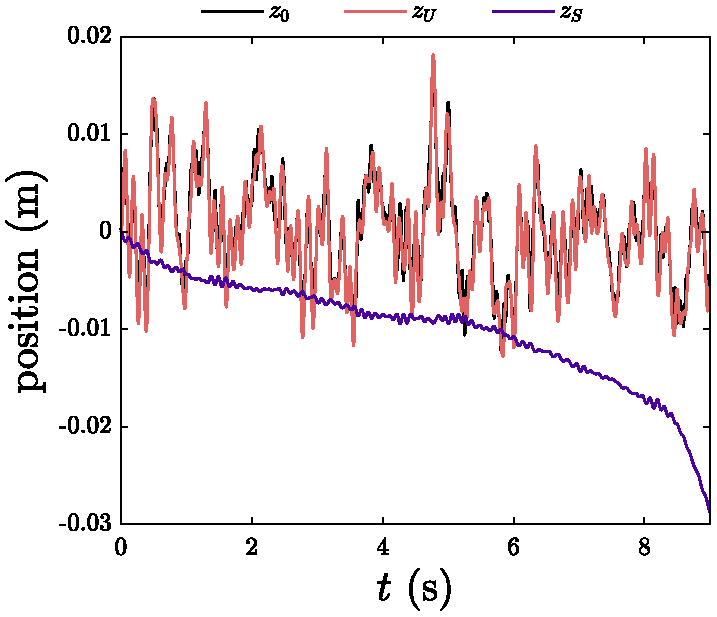
\includegraphics[width=\textwidth]{../ch8/figures/design2-position}
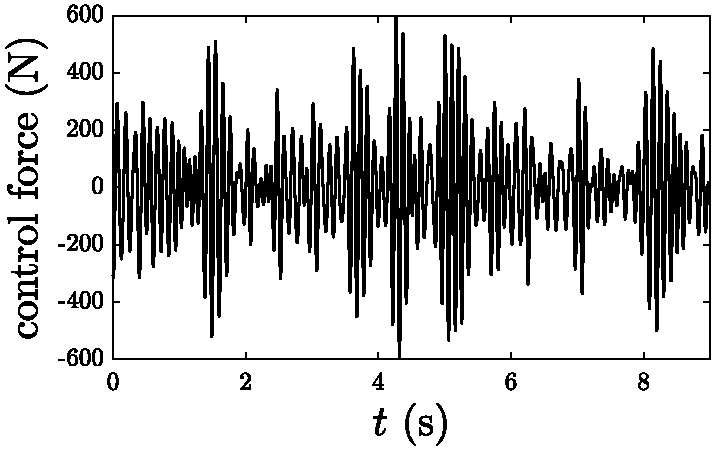
\includegraphics[width=\textwidth]{../ch8/figures/design2-control}
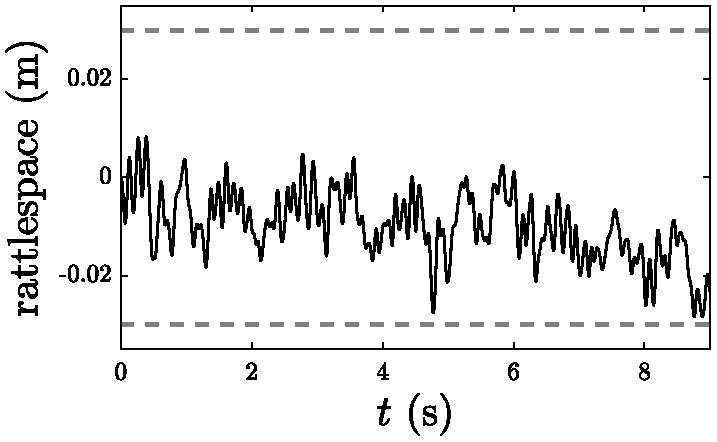
\includegraphics[width=\textwidth]{../ch8/figures/design2-rattlespace}
\caption{Pure active in Fig.~\ref{fig:ch8:csuspension2}.\label{fig:ch8:results2}}
\end{subfigure}%
\begin{subfigure}[b]{0.5\textwidth}
\centering
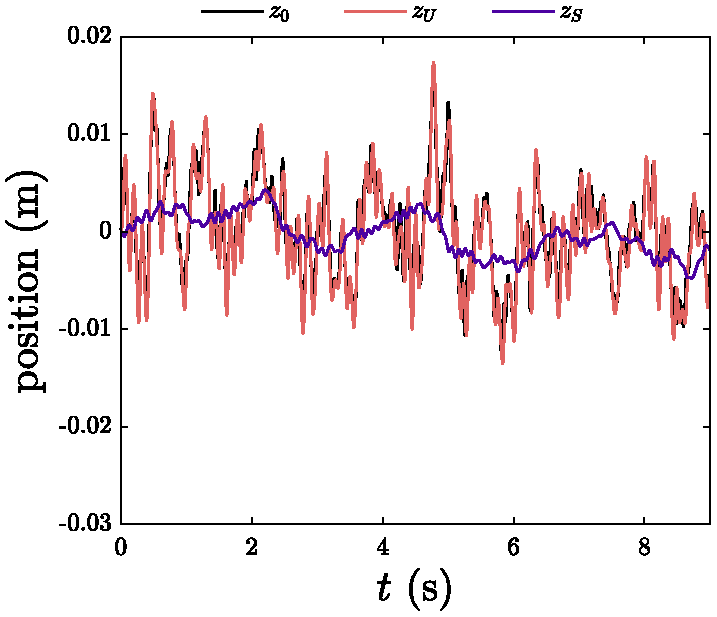
\includegraphics[width=\textwidth]{../ch8/figures/design1-position}
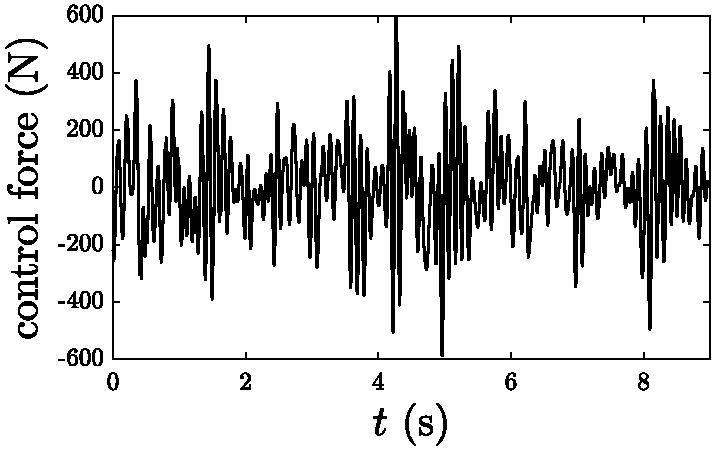
\includegraphics[width=\textwidth]{../ch8/figures/design1-control}
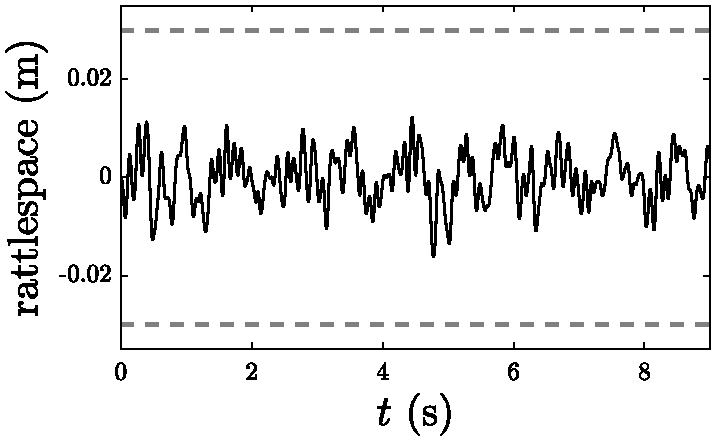
\includegraphics[width=\textwidth]{../ch8/figures/design1-rattlespace}
\caption{Canonical active in Fig.~\ref{fig:ch8:csuspension3}.\label{fig:ch8:results3}}
\end{subfigure}%

\caption{Optimal trajectories for two suspensions.}

\end{figure}

\begin{figure}

\begin{subfigure}[b]{0.5\textwidth}
\centering
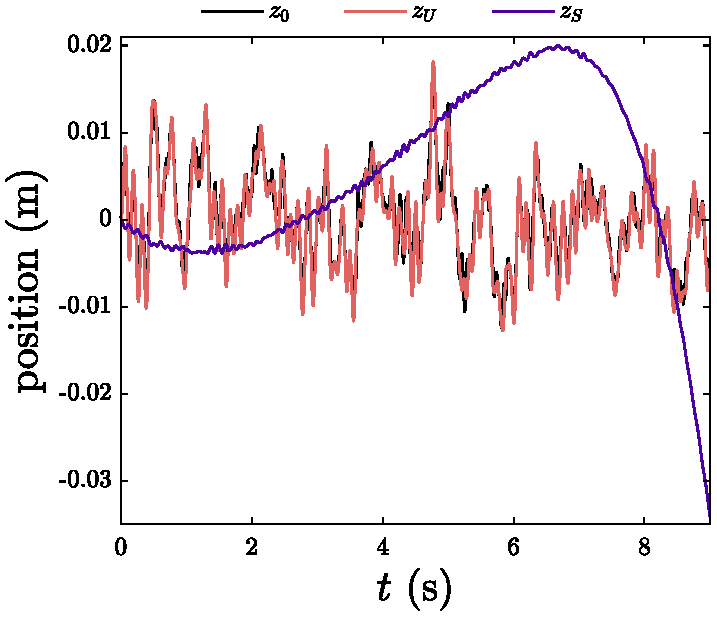
\includegraphics[width=\textwidth]{../ch8/figures/design4-position}
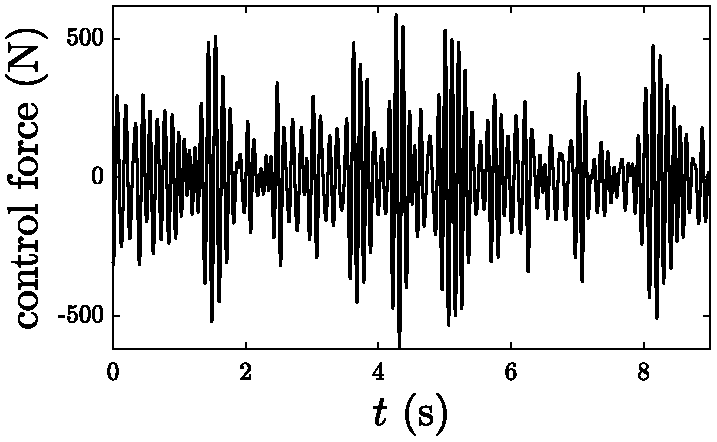
\includegraphics[width=\textwidth]{../ch8/figures/design4-control}
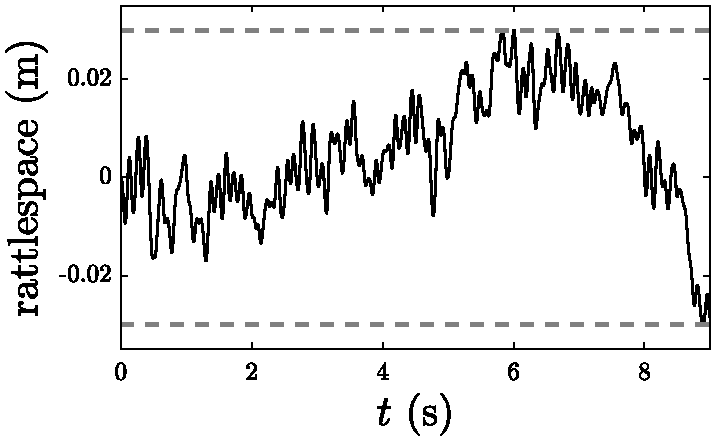
\includegraphics[width=\textwidth]{../ch8/figures/design4-rattlespace}
\caption{Active with dynamic absorber in Fig.~\ref{fig:ch8:csuspension4}.\label{fig:ch8:results4}}
\end{subfigure}%
\begin{subfigure}[b]{0.5\textwidth}
\centering
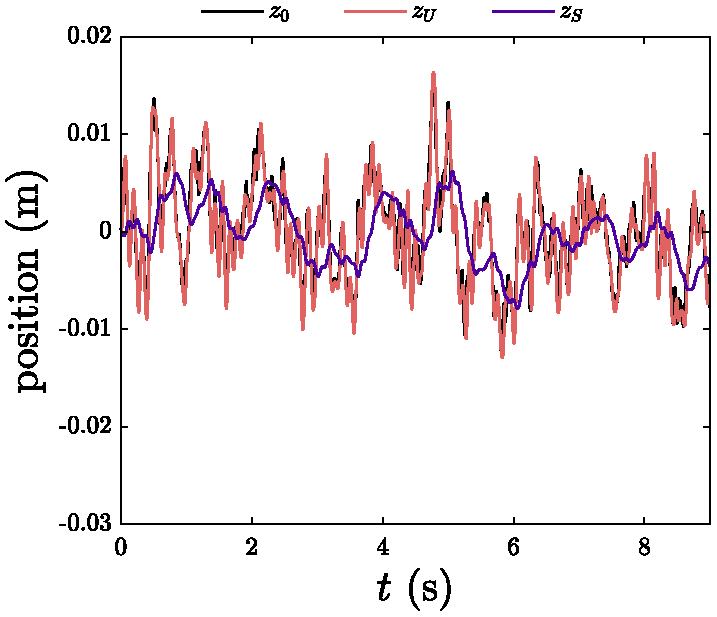
\includegraphics[width=\textwidth]{../ch8/figures/design5-position}
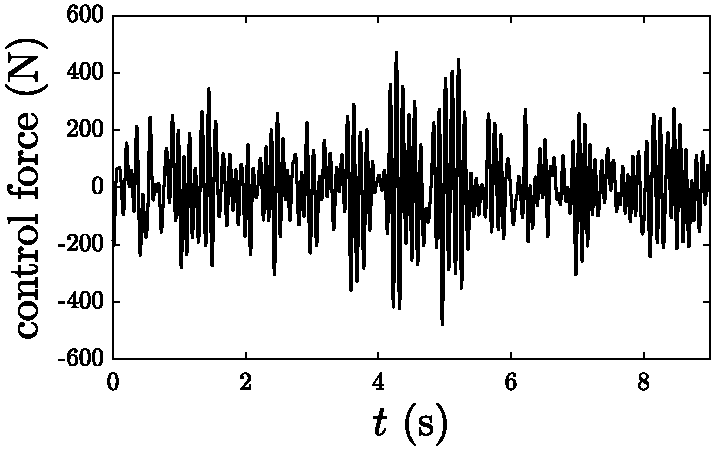
\includegraphics[width=\textwidth]{../ch8/figures/design5-control}
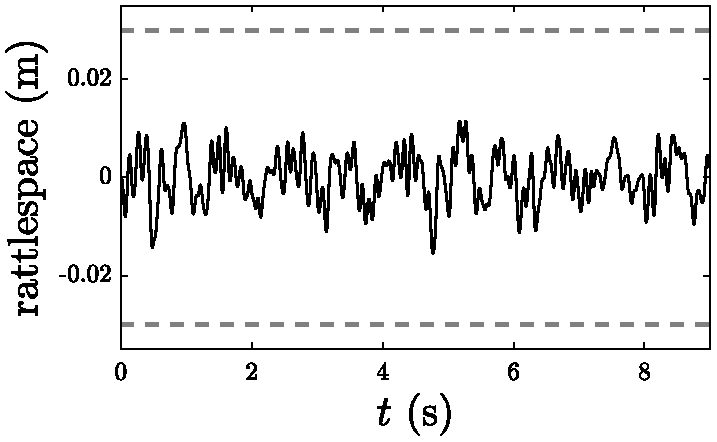
\includegraphics[width=\textwidth]{../ch8/figures/design5-rattlespace}
\caption{Active candidate in Fig.~\ref{fig:ch8:csuspension5}.\label{fig:ch8:results5}}
\end{subfigure}%

\caption{Optimal trajectories for two suspensions including the current best architecture.}

\end{figure}